\documentclass[12pt,aspectratio=169]{beamer}\usepackage[]{graphicx}\usepackage[]{xcolor}
% maxwidth is the original width if it is less than linewidth
% otherwise use linewidth (to make sure the graphics do not exceed the margin)
\makeatletter
\def\maxwidth{ %
  \ifdim\Gin@nat@width>\linewidth
    \linewidth
  \else
    \Gin@nat@width
  \fi
}
\makeatother

\definecolor{fgcolor}{rgb}{0.345, 0.345, 0.345}
\newcommand{\hlnum}[1]{\textcolor[rgb]{0.686,0.059,0.569}{#1}}%
\newcommand{\hlstr}[1]{\textcolor[rgb]{0.192,0.494,0.8}{#1}}%
\newcommand{\hlcom}[1]{\textcolor[rgb]{0.678,0.584,0.686}{\textit{#1}}}%
\newcommand{\hlopt}[1]{\textcolor[rgb]{0,0,0}{#1}}%
\newcommand{\hlstd}[1]{\textcolor[rgb]{0.345,0.345,0.345}{#1}}%
\newcommand{\hlkwa}[1]{\textcolor[rgb]{0.161,0.373,0.58}{\textbf{#1}}}%
\newcommand{\hlkwb}[1]{\textcolor[rgb]{0.69,0.353,0.396}{#1}}%
\newcommand{\hlkwc}[1]{\textcolor[rgb]{0.333,0.667,0.333}{#1}}%
\newcommand{\hlkwd}[1]{\textcolor[rgb]{0.737,0.353,0.396}{\textbf{#1}}}%
\let\hlipl\hlkwb

\usepackage{framed}
\makeatletter
\newenvironment{kframe}{%
 \def\at@end@of@kframe{}%
 \ifinner\ifhmode%
  \def\at@end@of@kframe{\end{minipage}}%
  \begin{minipage}{\columnwidth}%
 \fi\fi%
 \def\FrameCommand##1{\hskip\@totalleftmargin \hskip-\fboxsep
 \colorbox{shadecolor}{##1}\hskip-\fboxsep
     % There is no \\@totalrightmargin, so:
     \hskip-\linewidth \hskip-\@totalleftmargin \hskip\columnwidth}%
 \MakeFramed {\advance\hsize-\width
   \@totalleftmargin\z@ \linewidth\hsize
   \@setminipage}}%
 {\par\unskip\endMakeFramed%
 \at@end@of@kframe}
\makeatother

\definecolor{shadecolor}{rgb}{.97, .97, .97}
\definecolor{messagecolor}{rgb}{0, 0, 0}
\definecolor{warningcolor}{rgb}{1, 0, 1}
\definecolor{errorcolor}{rgb}{1, 0, 0}
\newenvironment{knitrout}{}{} % an empty environment to be redefined in TeX

\usepackage{alltt}

% Define the theme
\usepackage[sfmath]{kpfonts}
%\usepackage{fbb}
\usetheme[progressbar=frametitle, 
titleformat=smallcaps, 
titleformat section=smallcaps,
numbering=fraction]{metropolis}


% Load some packeges
\usepackage{appendixnumberbeamer}
\usepackage{dsfont}			% math font for ``double-bar'' ones
\usepackage{booktabs}
\usepackage{threeparttable, enumitem}
\usepackage{rotating}
\usepackage[scale=2]{ccicons}

\usepackage{bbding}
\usepackage{subfig}
\usepackage{graphicx}
\usepackage{epstopdf}
\usepackage{amssymb, amsmath}


\usepackage{xspace}
\newcommand{\themename}{\textbf{\textsc{metropolis}}\xspace}

% Package for fitting big tables to the slide
\usepackage{adjustbox}
\usepackage{multirow}
\usepackage{enumitem}

% Use American English APA quotations
\usepackage[american]{babel}     
\usepackage{csquotes}
\usepackage[
style=apa,
backend=biber,
maxcitenames=2,		
]{biblatex}
\DeclareLanguageMapping{american}{american-apa}
\uspunctuation

% Indicate bibliography file
\addbibresource{../notes/refs_workshop.bib}

% More bibliograpphy style settings
\AtEveryBibitem{
	\clearfield{labelmonth}
}
\setlength\bibhang{\parindent} % sets indentation in reference list; \parindent is default

% COSTUMIZE THE THEME
\definecolor{champagne}{RGB}{223, 227, 17}
\definecolor{coolblack}{RGB}{100, 39, 111}
\definecolor{hsggreen}{RGB}{0, 133, 63}
\definecolor{dimgrey}{RGB}{112,128,144}
\definecolor{ethblue}{RGB}{31,64,122}
\definecolor{ethorange}{RGB}{149,96,19}

% Change the progress bar color
\setbeamercolor{progress bar}{fg=ethorange} 
\setbeamercolor{title separator}{fg=ethorange}

\setbeamercolor{frametitle}{bg=ethblue} % sostituisci dimgrey qui
\setbeamercolor{alerted text}{%
	fg=ethorange
}
% Change thickness of progrss bar
\makeatletter
\setlength{\metropolis@progressinheadfoot@linewidth}{1.7pt}
\setlength{\metropolis@titleseparator@linewidth}{1.2pt}
\setlength{\metropolis@progressonsectionpage@linewidth}{1.2pt}

\setbeamertemplate{progress bar in section page}{
	\setlength{\metropolis@progressonsectionpage}{%
		\textwidth * \ratio{\thesection pt}{\totvalue{totalsection} pt}%
	}%
	\begin{tikzpicture}
		\fill[bg] (0,0) rectangle (\textwidth, \metropolis@progressonsectionpage@linewidth);
		\fill[fg] (0,0) rectangle (\metropolis@progressonsectionpage, \metropolis@progressonsectionpage@linewidth);
	\end{tikzpicture}%
}

\makeatother

\usepackage{totcount}

\newcounter{totalsection}
\regtotcounter{totalsection}

\AtBeginDocument{%
	\pretocmd{\section}{\refstepcounter{totalsection}}{\typeout{Yes, prepending was successful}}{\typeout{No, prepending was not it was successful}}%
}%


% Fancy question mark
\DeclareMathSymbol{\qm}{\mathalpha}{operators}{"3F}
\DeclareMathAlphabet{\mathbbold}{U}{bbold}{m}{n}

\titlegraphic{%
%	\includegraphics[width=.2\textwidth]{example-image-a}\hfill
%	\includegraphics[width=.2\textwidth]{example-image-b}\hfill
	\hfill
\includegraphics[width=.2\textwidth]{eth}
}

\makeatletter
\setbeamertemplate{title page}{
	\begin{minipage}[b][\paperheight]{\textwidth}
		\vfill%
		\ifx\inserttitle\@empty\else\usebeamertemplate*{title}\fi
		\ifx\insertsubtitle\@empty\else\usebeamertemplate*{subtitle}\fi
		\usebeamertemplate*{title separator}
		\ifx\beamer@shortauthor\@empty\else\usebeamertemplate*{author}\fi
		\ifx\insertdate\@empty\else\usebeamertemplate*{date}\fi
		\ifx\insertinstitute\@empty\else\usebeamertemplate*{institute}\fi
		\vfill
		\ifx\inserttitlegraphic\@empty\else\inserttitlegraphic\fi
		\vspace*{1cm}
	\end{minipage}
}
\makeatother

% Define smaller size than tiny
\makeatletter
\newcommand{\supertiny}{\@setfontsize{\supertiny}{5pt}{5pt}}
\makeatother

% Make non-current bullet points transparent
\setbeamercovered{transparent}

\usepackage{qtree}
\usepackage{tikz}
\usetikzlibrary{decorations.markings}
\usetikzlibrary{shapes.geometric}
\usetikzlibrary{decorations.pathreplacing}

\linespread{1.1}




%% Document starts -------------------------------------------------------------
\IfFileExists{upquote.sty}{\usepackage{upquote}}{}
\begin{document}


%%------------------------------------------------------------------------------

\section{Introduction}




\begin{frame}
\frametitle{Outline}

    \tableofcontents
    
\end{frame}


\begin{frame}
\frametitle{Introduction}

    \begin{alertblock}{About me}
    \small
    
    \begin{itemize}[itemsep=0em, topsep=0pt]
        \item Roberto Valli
        \item St. Gallen, ETH, UC Berkeley, ...?
        \item 3rd year @ ICR
        \item Nationalism, ethnic politics and sometimes partisanship
        \item I love panel data $<3$
    \end{itemize}

    \end{alertblock}

    \begin{alertblock}{Goals for today}
    \small

    \begin{itemize}[itemsep=0em, topsep=0pt]
        \item Give you an overview of DiD literature
        \item Discuss useful developments
        \item Help you choose the right model for your data
    \end{itemize}

    \end{alertblock}
%     
\end{frame}

%%------------------------------------------------------------------------------

\section{Basic DiD Dust-Off}


\begin{frame}
\frametitle{DiD setup}
    \centering\footnotesize


    \begin{tikzpicture}[scale=0.85, transform shape]
    \node  (0) at (-1, 7) {y};
    \node  (1) at (-1, -0) {}; %Origin
    \node  (2) at (10, -0) {t};
    \draw [->] (1.center) to (2);
    \draw [->] (1.center) to (0);
    \node  (10) at (2, -0.25) {0}; % periods
    \node  (11) at (5, -0.25) {1};
    \node  (11) at (8, -0.25) {2};
    % control group
    \fill (2, 1.5) circle (2pt) node[left=2pt] {$Y_{i1}(0)\ | \ D = 0$};
    % \node  (3) at (2, 1.5) {$Y_{i1}(0)\ | \ D = 0$};
    \fill (5, 2) circle (2pt) node[above=2pt] {$Y_{i2}(0)\ | \ D = 0$};
    % \node  (4) at (5, 2) {$Y_{i2}(0)\ | \ D = 0$};
    % \fill (8, 1) circle (2pt) node[right=2pt] {$Y_{i3}(0)\ | \ D = 0$};
    % \node  (5) at (8, 1) {$Y_{i3}(0)\ | \ D = 0$};
    % \draw [thick] (8, 1) to (5, 2);
    \draw [thick] (5, 2) to (2, 1.5);
    % treatment group (observed)
    \fill (2, 4) circle (2pt) node[left=2pt] {$Y_{i1}(1)\ | \ D = 1$};
    % \node  (6) at (2, 4) {$Y_{i1}(1)\ | \ D = 1$};
    \fill (5, 6) circle (2pt) node[above=2pt] {$Y_{i2}(1)\ | \ D = 1$};
    % \node  (7) at (5, 6) {$Y_{i2}(1)\ | \ D = 1$};
    \draw [thick] (5, 6) to (2, 4);
    % treatment group (counterfactual)

    \end{tikzpicture}
    
\end{frame}

\begin{frame}
\frametitle{Counterfactual outcome}
    \centering\footnotesize
    
    \begin{tikzpicture}[scale=0.85, transform shape]
    \node  (0) at (-1, 7) {y};
    \node  (1) at (-1, -0) {}; %Origin
    \node  (2) at (10, -0) {t};
    \draw [->] (1.center) to (2);
    \draw [->] (1.center) to (0);
    \node  (10) at (2, -0.25) {0}; % periods
    \node  (11) at (5, -0.25) {1};
    % \node  (11) at (8, -0.25) {2};
    % control group
    \fill (2, 1.5) circle (2pt) node[left=2pt] {$Y_{i1}(0)\ | \ D = 0$};
    % \node  (3) at (2, 1.5) {$Y_{i1}(0)\ | \ D = 0$};
    \fill (5, 2) circle (2pt) node[above=2pt] {$Y_{i2}(0)\ | \ D = 0$};
    % \node  (4) at (5, 2) {$Y_{i2}(0)\ | \ D = 0$};
    % \fill (8, 1) circle (2pt) node[right=2pt] {$Y_{i3}(0)\ | \ D = 0$};
    % \node  (5) at (8, 1) {$Y_{i3}(0)\ | \ D = 0$};
    % \draw [thick] (8, 1) to (5, 2);
    \draw [thick] (5, 2) to (2, 1.5);
    % treatment group (observed)
    \fill (2, 4) circle (2pt) node[left=2pt] {$Y_{i1}(1)\ | \ D = 1$};
    % \node  (6) at (2, 4) {$Y_{i1}(1)\ | \ D = 1$};
    \fill (5, 6) circle (2pt) node[above=2pt] {$Y_{i2}(1)\ | \ D = 1$};
    % \node  (7) at (5, 6) {$Y_{i2}(1)\ | \ D = 1$};
    % \fill (8, 5.5) circle (2pt) node[right=2pt] {$Y_{i3}(1)\ | \ D = 1$};
    % \node  (8) at (8, 5.5) {$Y_{i3}(1)\ | \ D = 1$};
    \draw [thick] (5, 6) to (2, 4);
    % \draw [thick] (8, 5.5) to (5, 6);
    % treatment group (counterfactual)
    \fill (5, 4.5) circle (2pt) node[above=2pt] {$Y_{i2}(0)\ | \ D = 1$};
    % \fill (8, 3.5) circle (2pt) node[right=2pt] {$Y_{i3}(0)\ | \ D = 1$};
    % \node  (12) at (8, 3.5) {$Y_{i3}(0)\ | \ D = 1$};
    % \draw [dash dot] (8, 3.5) to (5, 4.5);
    \draw [dash dot] (5, 4.5) to (2, 4);
    \end{tikzpicture}
\end{frame}


\begin{frame}
\frametitle{Inference with DiD}
    \centering\footnotesize
    
    \begin{tikzpicture}[scale=0.85, transform shape]
    \node  (0) at (-1, 7) {y};
    \node  (1) at (-1, -0) {}; %Origin
    \node  (2) at (10, -0) {t};
    \draw [->] (1.center) to (2);
    \draw [->] (1.center) to (0);
    \node  (10) at (2, -0.25) {0}; % periods
    \node  (11) at (5, -0.25) {1};
    % \node  (11) at (8, -0.25) {2};
    % control group
    \fill (2, 1.5) circle (2pt) node[left=2pt] {$Y_{i1}(0)\ | \ D = 0$};
    % \node  (3) at (2, 1.5) {$Y_{i1}(0)\ | \ D = 0$};
    \fill (5, 2) circle (2pt) node[above=2pt] {$Y_{i2}(0)\ | \ D = 0$};
    % \node  (4) at (5, 2) {$Y_{i2}(0)\ | \ D = 0$};
    % \fill (8, 1) circle (2pt) node[right=2pt] {$Y_{i3}(0)\ | \ D = 0$};
    % \node  (5) at (8, 1) {$Y_{i3}(0)\ | \ D = 0$};
    % \draw [thick] (8, 1) to (5, 2);
    \draw [thick] (5, 2) to (2, 1.5);
    % treatment group (observed)
    \fill (2, 4) circle (2pt) node[left=2pt] {$Y_{i1}(1)\ | \ D = 1$};
    % \node  (6) at (2, 4) {$Y_{i1}(1)\ | \ D = 1$};
    \fill (5, 6) circle (2pt) node[above=2pt] {$Y_{i2}(1)\ | \ D = 1$};
    % \node  (7) at (5, 6) {$Y_{i2}(1)\ | \ D = 1$};
    % \fill (8, 5.5) circle (2pt) node[right=2pt] {$Y_{i3}(1)\ | \ D = 1$};
    % \node  (8) at (8, 5.5) {$Y_{i3}(1)\ | \ D = 1$};
    \draw [thick] (5, 6) to (2, 4);
    % \draw [thick] (8, 5.5) to (5, 6);
    % treatment group (counterfactual)
    \fill (5, 4.5) circle (2pt) node[above=2pt] {$Y_{i2}(0)\ | \ D = 1$};
    % \fill (8, 3.5) circle (2pt) node[right=2pt] {$Y_{i3}(0)\ | \ D = 1$};
    % \node  (12) at (8, 3.5) {$Y_{i3}(0)\ | \ D = 1$};
    % \draw [dash dot] (8, 3.5) to (5, 4.5);
    \draw [dash dot] (5, 4.5) to (2, 4);
    % legend
    \node  (13) at (9.5, 4.5) {%
    $\begin{aligned}
    \tau = & E\left[ Y_{i2}(1) - Y_{i1}(1) \ | \ D = 1\right] -\\ 
           & E\left[ Y_{i2}(0) - Y_{i1}(0) \ | \ D = 0\right]
    \end{aligned}$
    };
    \end{tikzpicture}
\end{frame}


\begin{frame}
\frametitle{Three-period DiD}

    \centering\footnotesize
    \begin{tikzpicture}[scale=0.85, transform shape]
    \node  (0) at (-1, 7) {y};
    \node  (1) at (-1, -0) {}; %Origin
    \node  (2) at (10, -0) {t};
    \draw [->] (1.center) to (2);
    \draw [->] (1.center) to (0);
    \node  (10) at (2, -0.25) {0}; % periods
    \node  (11) at (5, -0.25) {1};
    \node  (11) at (8, -0.25) {2};
    % control group
    \fill (2, 1.5) circle (2pt) node[left=2pt] {$Y_{i1}(0)\ | \ D = 0$};
    % \node  (3) at (2, 1.5) {$Y_{i1}(0)\ | \ D = 0$};
    \fill (5, 2) circle (2pt) node[above=2pt] {$Y_{i2}(0)\ | \ D = 0$};
    % \node  (4) at (5, 2) {$Y_{i2}(0)\ | \ D = 0$};
    \fill (8, 1) circle (2pt) node[right=2pt] {$Y_{i3}(0)\ | \ D = 0$};
    % \node  (5) at (8, 1) {$Y_{i3}(0)\ | \ D = 0$};
    \draw [thick] (8, 1) to (5, 2);
    \draw [thick] (5, 2) to (2, 1.5);
    % treatment group (observed)
    \fill (2, 4) circle (2pt) node[left=2pt] {$Y_{i1}(1)\ | \ D = 1$};
    % \node  (6) at (2, 4) {$Y_{i1}(1)\ | \ D = 1$};
    \fill (5, 6) circle (2pt) node[above=2pt] {$Y_{i2}(1)\ | \ D = 1$};
    % \node  (7) at (5, 6) {$Y_{i2}(1)\ | \ D = 1$};
    \fill (8, 5.5) circle (2pt) node[right=2pt] {$Y_{i3}(1)\ | \ D = 1$};
    % \node  (8) at (8, 5.5) {$Y_{i3}(1)\ | \ D = 1$};
    \draw [thick] (5, 6) to (2, 4);
    \draw [thick] (8, 5.5) to (5, 6);
    % treatment group (counterfactual)
    \fill (5, 4.5) circle (2pt) node[above=2pt] {$Y_{i2}(0)\ | \ D = 1$};
    \fill (8, 3.5) circle (2pt) node[right=2pt] {$Y_{i3}(0)\ | \ D = 1$};
    % \node  (12) at (8, 3.5) {$Y_{i3}(0)\ | \ D = 1$};
    \draw [dash dot] (8, 3.5) to (5, 4.5);
    \draw [dash dot] (5, 4.5) to (2, 4);
    % other
    \end{tikzpicture}
\end{frame}


\begin{frame}
\frametitle{The brilliance of DiDs}

    \begin{alertblock}{Inferential problem}
    \small

    \begin{itemize}[itemsep=0em, topsep=0pt]
        \item Counterfactual outcomes as \textbf{missing data}
        \item How to produce valid counterfactual outcome $\hat{Y}(0)| D = 1$?
        \item $\rightarrow$ Find unbiased function $g(Y)$, s.t.  $E[ \hat{Y}(0)| D = 1 -  Y(0)| D = 1] = 0$
        \item $\rightarrow$ Exploit parallel trends assumption and SUTVA
    \end{itemize}

    \end{alertblock}

    \begin{alertblock}{Solutions in basic DiD}
    \small

    \begin{itemize}[itemsep=0em, topsep=0pt]
        \item Traditionally, use linear $g(\dot)$ on \textbf{all} within-individual variation.
        \item All ITEs need to have same weight
        \item Easily estimated with TWFE, DiM, first-difference
    \end{itemize}

    \end{alertblock}

\end{frame}

%%------------------------------------------------------------------------------

\section{Limitations of basic DiD setting }

\begin{frame}
\frametitle{The breakthrough}

    \begin{alertblock}{Mid 2010s}
    \small

    \begin{itemize}[itemsep=0em, topsep=0pt]
        \item Econometricians question the validity of TWFE
        \item Main culprit: DiD with staggered adoption.\\{\footnotesize (e.g., Goodman-Bacon 2021, Sun and Abrams 2021, Callaway and Sant'Anna 2021}
        \item $\rightarrow$ Econometric lit. kinda left applied research behind \dots
    \end{itemize}

    \end{alertblock}

    \begin{alertblock}{Problems identified}
    \small

    \begin{itemize}[itemsep=0em, topsep=0pt]
        \item Researchers refer to theory of 2-period DiD, do completely different things.
        \item TWFE makes problematic comparisons.
        \item Overall TWFE ATT is weighted average of cohort-specific ATTs.
        \item $\rightarrow$ Cohort-ATTs can get weird weights.
        \item Pre-trends tests are underpowered, but also give false rejections
        % \item Your turn!
        % \item Wrap  up
    \end{itemize}

    \end{alertblock}

\end{frame}



%%------------------------------------------------------------------------------

\section{New Approaches to DiD}


\begin{frame}[fragile]
    \frametitle{Example: Non-absorbing state treatment}
    \scriptsize\centering

    \resizebox{0.7\textwidth}{!}{
            \Tree[. [.{N. treated units $>$ 1} [.{T = 2} {Classic DiD\\ (Sec. 4.2)} ]
                                   [.{T $>$ 2} [.{Non-absorbing state\\ treatment} { {\texttt{GSC} (Sec. 4.43)}\\ {\texttt{fect} (Sec. 4.42)}\\ {\texttt{PanelMatch} (Sec. 4.43)} } ]
                                             [.{Absorbing-state\\ treatment}
                                                                              [.{Staggered\\ treatment}  { \texttt{did, did2s,}\\ \texttt{didimputation},\\ \texttt{DRDID, fixest},\\ \texttt{wfe} (Sec. 4.3.1-2)} ]
                                                                              [.{Contemporaneous\\ treatment} {Classic DiD with multiple\\ periods (Sec 4.3.1)} ]]]]
                    [.{N. treated units = 1} [.{SCM\\ (Sec. 4.1)} ]]
                  ]
    }

\end{frame}


\begin{frame}[fragile]
    \frametitle{Go-to packages in (early) 2023}


    \begin{alertblock}{Staggered DiD settings}
    \small

    \begin{itemize}[itemsep=0em, topsep=0pt]
        \item \texttt{did} package
    \end{itemize}

    \end{alertblock}

    \begin{alertblock}{Non-absorbing state DiDs}
    \small

    \begin{itemize}[itemsep=0em, topsep=0pt]
        \item \texttt{felm} package
        \item \texttt{PanelMatch} package
    \end{itemize}

    \end{alertblock}
    \small

\begin{knitrout}
\definecolor{shadecolor}{rgb}{0.969, 0.969, 0.969}\color{fgcolor}\begin{kframe}
\begin{alltt}
\hlcom{# Load packages}
\hlkwd{library}\hlstd{(tidyverse)}
\hlkwd{library}\hlstd{(fixest)}
\hlkwd{library}\hlstd{(did)}
\hlkwd{library}\hlstd{(fect)}
\hlkwd{library}\hlstd{(PanelMatch)}
\end{alltt}
\end{kframe}
\end{knitrout}

\end{frame}


\begin{frame}[fragile]
    \frametitle{Example: Staggered treatment}
    \scriptsize
\begin{knitrout}
\definecolor{shadecolor}{rgb}{0.969, 0.969, 0.969}\color{fgcolor}

{\centering 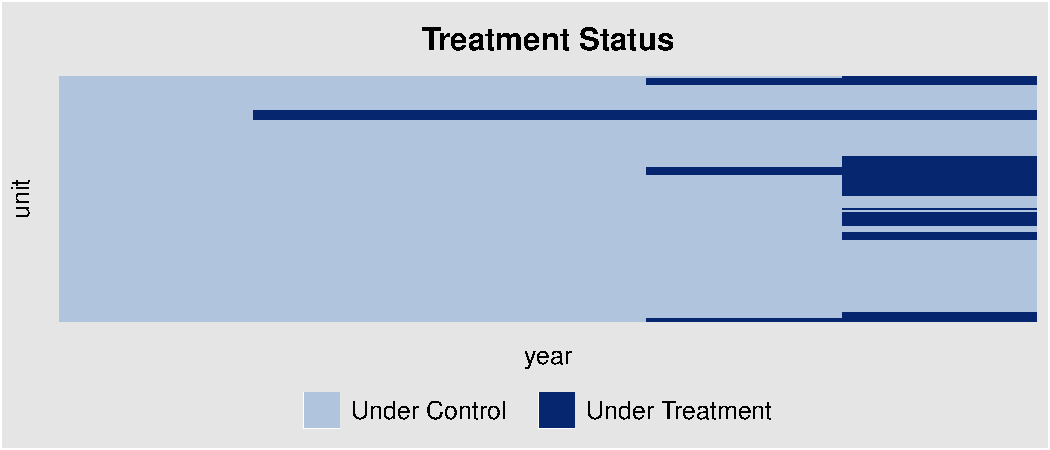
\includegraphics[width=\maxwidth]{figure/unnamed-chunk-3-1} 

}


\end{knitrout}

\end{frame}


\begin{frame}[fragile]
    \frametitle{Example: Staggered treatment}
    \scriptsize
\begin{knitrout}
\definecolor{shadecolor}{rgb}{0.969, 0.969, 0.969}\color{fgcolor}\begin{kframe}
\begin{alltt}
\hlcom{# Fit models}
\hlstd{mod_twfe} \hlkwb{<-} \hlkwd{feols}\hlstd{(lemp} \hlopt{~} \hlstd{post} \hlopt{|} \hlstd{countyreal} \hlopt{+} \hlstd{year, dat_did)}
\hlstd{mod_nvt} \hlkwb{<-} \hlkwd{att_gt}\hlstd{(}\hlstr{"lemp"}\hlstd{,} \hlstr{"year"}\hlstd{,} \hlstr{"countyreal"}\hlstd{,} \hlstr{"first.treat"}\hlstd{,}
                  \hlkwc{data} \hlstd{= dat_did,} \hlkwc{control_group} \hlstd{=} \hlstr{"nevertreated"}\hlstd{)}
\hlstd{mod_nyt} \hlkwb{<-} \hlkwd{att_gt}\hlstd{(}\hlstr{"lemp"}\hlstd{,} \hlstr{"year"}\hlstd{,} \hlstr{"countyreal"}\hlstd{,} \hlstr{"first.treat"}\hlstd{,}
                  \hlkwc{data} \hlstd{= dat_did,} \hlkwc{control_group} \hlstd{=} \hlstr{"notyettreated"}\hlstd{)}
\end{alltt}
\end{kframe}
\end{knitrout}
    
\end{frame}


\begin{frame}[fragile]
    \frametitle{Example: Staggered treatment cont'd}
    \scriptsize
\begin{knitrout}
\definecolor{shadecolor}{rgb}{0.969, 0.969, 0.969}\color{fgcolor}\begin{kframe}
\begin{alltt}
\hlcom{# Compare estimates}
\hlkwd{data.frame}\hlstd{(}\hlkwc{twfe} \hlstd{= mod_twfe}\hlopt{$}\hlstd{coefficients,}
           \hlstr{"did never"} \hlstd{=} \hlkwd{aggte}\hlstd{(mod_nvt,} \hlkwc{type} \hlstd{=} \hlstr{"simple"}\hlstd{)}\hlopt{$}\hlstd{overall.att,}
           \hlstr{"did notyet"} \hlstd{=} \hlkwd{aggte}\hlstd{(mod_nyt,} \hlkwc{type} \hlstd{=} \hlstr{"simple"}\hlstd{)}\hlopt{$}\hlstd{overall.att)}
\end{alltt}
\begin{verbatim}
##             twfe   did.never  did.notyet
## post -0.03654894 -0.03995128 -0.03976363
\end{verbatim}
\end{kframe}
\end{knitrout}
     

    \begin{alertblock}{Insights}
    \small

    \begin{itemize}[itemsep=0em, topsep=0pt]
        \item TWFE's bias is generally conservative
    \end{itemize}

    \end{alertblock}
\end{frame}


\begin{frame}[fragile]
    \frametitle{Example: Non-absorbing state}
    \scriptsize
\begin{knitrout}
\definecolor{shadecolor}{rgb}{0.969, 0.969, 0.969}\color{fgcolor}

{\centering 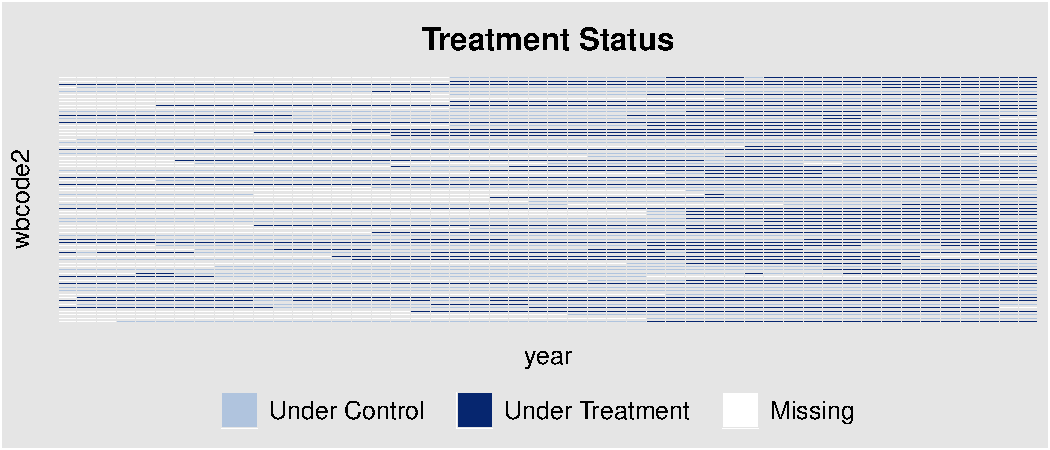
\includegraphics[width=\maxwidth]{figure/unnamed-chunk-6-1} 

}


\end{knitrout}
     

\end{frame}


\begin{frame}[fragile]
    \frametitle{Example: Non-absorbing state treatment}
    \scriptsize
    
\begin{knitrout}
\definecolor{shadecolor}{rgb}{0.969, 0.969, 0.969}\color{fgcolor}\begin{kframe}
\begin{alltt}
\hlcom{# Fit baseline model}
\hlstd{mod_twfe} \hlkwb{<-} \hlkwd{feols}\hlstd{(y} \hlopt{~} \hlstd{dem} \hlopt{|} \hlstd{wbcode2} \hlopt{+} \hlstd{year, dat_dem)}

\hlcom{# Fit other models}
\hlstd{mod_ife} \hlkwb{<-} \hlkwd{fect}\hlstd{(y} \hlopt{~} \hlstd{dem , dat_dem,} \hlkwc{index} \hlstd{=} \hlkwd{c}\hlstd{(}\hlstr{"wbcode2"}\hlstd{,} \hlstr{"year"}\hlstd{),} \hlkwc{se} \hlstd{= F,}
                 \hlkwc{method} \hlstd{=} \hlstr{"ife"}\hlstd{,} \hlkwc{na.rm} \hlstd{= T)}
\hlstd{mod_mc} \hlkwb{<-} \hlkwd{fect}\hlstd{(y} \hlopt{~} \hlstd{dem , dat_dem,} \hlkwc{index} \hlstd{=} \hlkwd{c}\hlstd{(}\hlstr{"wbcode2"}\hlstd{,} \hlstr{"year"}\hlstd{),} \hlkwc{se} \hlstd{= F,}
                 \hlkwc{method} \hlstd{=} \hlstr{"mc"}\hlstd{,} \hlkwc{na.rm} \hlstd{= T)}
\hlstd{matched} \hlkwb{<-} \hlkwd{PanelMatch}\hlstd{(}\hlkwc{lag} \hlstd{=} \hlnum{5}\hlstd{,} \hlkwc{lead} \hlstd{=} \hlnum{0}\hlopt{:}\hlnum{5}\hlstd{,} \hlkwc{unit.id} \hlstd{=} \hlstr{"wbcode2"}\hlstd{,} \hlkwc{time.id} \hlstd{=} \hlstr{"year"}\hlstd{,}
                      \hlkwc{covs.formula} \hlstd{=} \hlopt{~}\hlkwd{I}\hlstd{(}\hlkwd{lag}\hlstd{(y,} \hlnum{1}\hlopt{:}\hlnum{4}\hlstd{)),}
                      \hlkwc{treatment} \hlstd{=} \hlstr{"dem"}\hlstd{,} \hlkwc{outcome.var} \hlstd{=} \hlstr{"y"}\hlstd{,} \hlkwc{qoi} \hlstd{=} \hlstr{"att"}\hlstd{,}
                      \hlkwc{data} \hlstd{= dat_dem,} \hlkwc{refinement.method} \hlstd{=} \hlstr{"mahalanobis"}\hlstd{)}
\hlstd{mod_pm} \hlkwb{<-} \hlkwd{PanelEstimate}\hlstd{(matched, dat_dem,} \hlkwc{pooled} \hlstd{= T)}
\end{alltt}
\end{kframe}
\end{knitrout}
     

\end{frame}


\begin{frame}[fragile]
    \frametitle{Example: Non-absorbing state treatment cont'd}
    \scriptsize
    
\begin{knitrout}
\definecolor{shadecolor}{rgb}{0.969, 0.969, 0.969}\color{fgcolor}\begin{kframe}
\begin{alltt}
\hlcom{# Compare estimates}
\hlkwd{data.frame}\hlstd{(}\hlkwc{twfe} \hlstd{=} \hlkwd{as.numeric}\hlstd{(mod_twfe}\hlopt{$}\hlstd{coefficients[}\hlnum{1}\hlstd{]),}
           \hlstr{"fect ife"} \hlstd{=} \hlkwd{as.numeric}\hlstd{(mod_ife}\hlopt{$}\hlstd{att.avg),}
           \hlstr{"fect mc"} \hlstd{=} \hlkwd{as.numeric}\hlstd{(mod_mc}\hlopt{$}\hlstd{att.avg),}
           \hlstr{"panelmatch"} \hlstd{=} \hlkwd{as.numeric}\hlstd{(}\hlkwd{summary}\hlstd{(mod_pm)}\hlopt{$}\hlstd{summary[,} \hlnum{1}\hlstd{]))}
\end{alltt}
\begin{verbatim}
## Weighted Difference-in-Differences with Mahalanobis Distance
## Matches created with 5 lags
## 
## Standard errors computed with 1000 Weighted bootstrap samples
## 
## Estimate of Average Treatment Effect on the Treated (ATT) by Period:
##        twfe fect.ife fect.mc panelmatch
## 1 -10.11222 1.214884 2.08486    1.84098
\end{verbatim}
\end{kframe}
\end{knitrout}
     

\end{frame}


\begin{frame}[fragile]
    \frametitle{Example: Non-absorbing state treatment cont'd}
    \scriptsize
    
\begin{knitrout}
\definecolor{shadecolor}{rgb}{0.969, 0.969, 0.969}\color{fgcolor}

{\centering 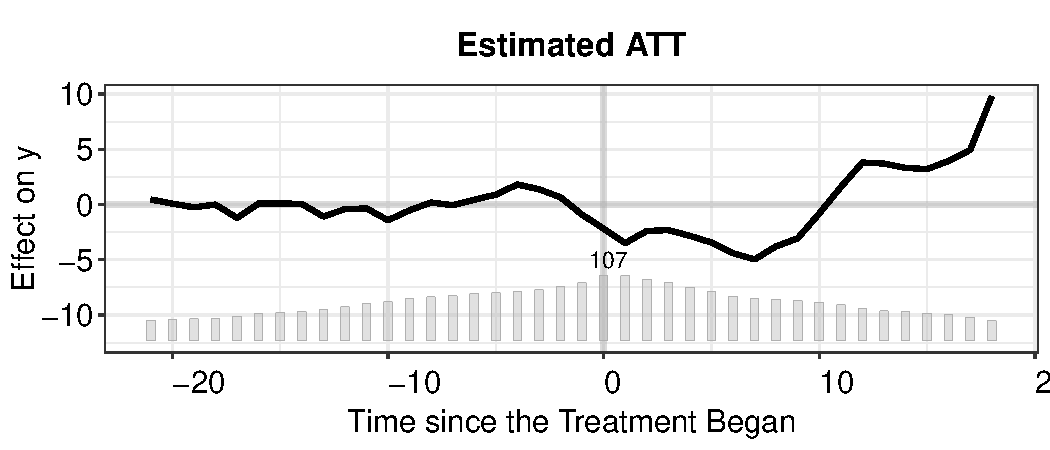
\includegraphics[width=0.49\linewidth]{figure/unnamed-chunk-9-1} 
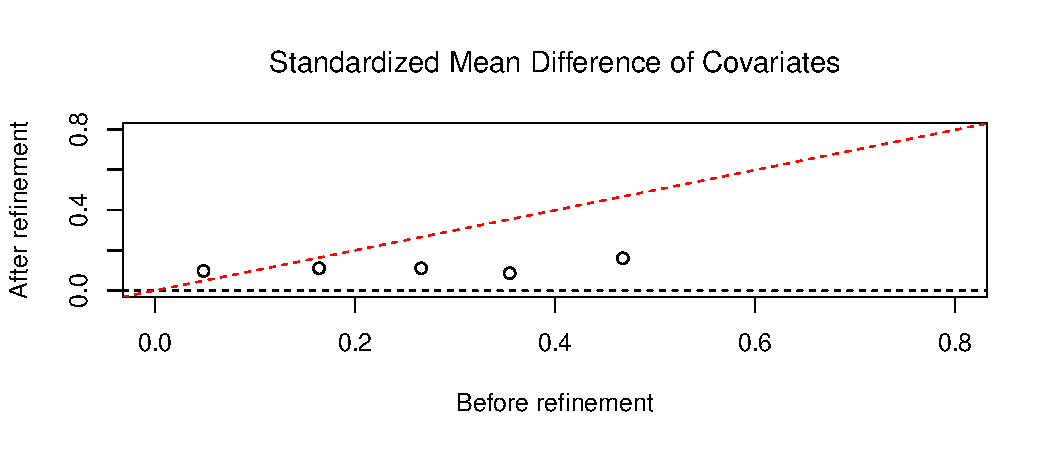
\includegraphics[width=0.49\linewidth]{figure/unnamed-chunk-9-2} 

}


\end{knitrout}
     

\end{frame}



%%------------------------------------------------------------------------------

\section{Your Turn!}


\begin{frame}
\frametitle{Tell us your data struggles}

    \begin{alertblock}{}

    \begin{itemize}
        \item Do you work with TSCS data?
        \item Have you encountered limitations in TWFE models?
        \item Has the absence of methods held you from researching sth?
        \item $\dots$ 
    \end{itemize}

    \end{alertblock}

\end{frame}

%%------------------------------------------------------------------------------

\section{Wrap-up}


\begin{frame}
\frametitle{DiD as prediction exercise}

    \begin{alertblock}{Problems with estimation led to rethink DiD}

    \begin{itemize}[itemsep=0em, topsep=0pt]
    \small
        \item Counterfactual outcomes as \textbf{non-linear prediction task}
        \item $\rightarrow$ Generalized synthetic control
        \item Counterfactual outcomes as \textbf{missing data}
        \item $\rightarrow$ Matrix completion method
        \item Counterfactual outcomes as \textbf{matching problem}
        \item $\rightarrow$ PanelMatch method
    \end{itemize}

    \end{alertblock}

    \begin{alertblock}{Outcome of the literature}

    \begin{itemize}[itemsep=0em, topsep=0pt]
    \small
        \item Different perspectives led to different solutions to problems.
        \item Broad set of concrete tools to apply DiD logic in broad set of cases.
        \item Great set of R packages!
    \end{itemize}

    \end{alertblock}

\end{frame}


\begin{frame}
\frametitle{Debate: Let's talk causality!}

    \begin{alertblock}{How causality is often discussed}

    \begin{itemize}[itemsep=0em, topsep=0pt]
    \small
        \item Your $X$ is not exogenous to $Y$: I don't believe you.
        \item There might be confounders: I don't believe you.
        \item $\rightarrow$ If a statistic is not \textbf{unbiased}, it might be anything.
        % \item Counterfactual outcomes as \textbf{matching problem}
        % \item $\rightarrow$ PanelMatch method
    \end{itemize}

    \end{alertblock}

    \begin{alertblock}{A better way of discussing causality (?)}

    \begin{itemize}[itemsep=0em, topsep=0pt]
    \small
        \item Your estimate is confounded: What is the chance that your results have another sign?
        \item Your $X$ is not exogenous: Are you sure the variation means what you argue?
        \item What kind of bias do you have, and what does it tell on the "true" $\tau$?
        \item $\rightarrow$ Focus on substantive meaning of estimates and biases!
    \end{itemize}

    \end{alertblock}

\end{frame}


\end{document}
